\documentclass{article}

% if you need to pass options to natbib, use, e.g.:
% \PassOptionsToPackage{numbers, compress}{natbib}
% before loading nips_2017
%
% to avoid loading the natbib package, add option nonatbib:
% \usepackage[nonatbib]{nips_2017}
\usepackage{nips_2017}

\RequirePackage[l2tabu, orthodox]{nag}
\documentclass{article}

% FONTS
\usepackage[T1]{fontenc}

% Replace default Latin Modern typewriter with its proportional counterpart
% http://www.tug.dk/FontCatalogue/lmoderntypewriterprop/
\renewcommand*\ttdefault{lmvtt}


%%% OPTION 1 - Fourier Math + New Century Schoolbook + ParaType Sans

% % Import Fourier Math (this imposes its own New Century Schoolbook type)
% % http://www.ctan.org/tex-archive/fonts/fouriernc/
%\usepackage{fouriernc}
%\usepackage{amsmath}
% % Replace with TeX Gyre Schola version of New Century Schoolbook (must scale!)
% % http://www.tug.dk/FontCatalogue/tgschola/
%\usepackage[scale=0.92]{tgschola}
%\usepackage[scaled=0.88]{PTSans}

%% OPTION 2 - MathDesign Math + Bitstream Charter + ParaType Sans

% Import MathDesign (this brings along Bitstream Charter)
% http://www.ctan.org/tex-archive/fonts/mathdesign/
\usepackage[bitstream-charter]{mathdesign}
\usepackage{amsmath}
\usepackage[scaled=0.92]{PTSans}


% %%% OPTION 3 - MTPRO 2 Math + Termes Times + ParaType Sans

% \usepackage{tgtermes}
% \usepackage{amsmath}
% \usepackage[subscriptcorrection,
%             amssymbols,
%             mtpbb,
%             mtpcal,
%             nofontinfo  % suppresses all warnings
%            ]{mtpro2}
% \usepackage{scalefnt,letltxmacro}
% \LetLtxMacro{\oldtextsc}{\textsc}
% \renewcommand{\textsc}[1]{\oldtextsc{\scalefont{1.10}#1}}
% \usepackage[scaled=0.92]{PTSans}

% GEOMETRY
\usepackage[
  paper  = letterpaper,
  left   = 1.65in,
  right  = 1.65in,
  top    = 1.0in,
  bottom = 1.0in,
  ]{geometry}

% COLOR
\usepackage[usenames,dvipsnames]{xcolor}
\definecolor{shadecolor}{gray}{0.9}

% SPACING and TEXT
\usepackage[final,expansion=alltext]{microtype}
\usepackage[english]{babel}
\usepackage[parfill]{parskip}
\usepackage{afterpage}
\usepackage{framed}
\usepackage{verbatim}

%redefine the leftbar environment to accept a width and coloring options
\renewenvironment{leftbar}[1][\hsize]
{%
  \def\FrameCommand
  {%
    {\color{Gray}\vrule width 3pt}%
    \hspace{10pt}%
    %\hspace{0pt}\fboxsep=\FrameSep\colorbox{black!10}%
  }%
  \MakeFramed{\hsize#1\advance\hsize-\width\FrameRestore}%
}%
{\endMakeFramed}

% define a paragraph header function
\DeclareRobustCommand{\parhead}[1]{\textbf{#1}~}

% EDITING
% line numbering in left margin
\usepackage{lineno}
\renewcommand\linenumberfont{\normalfont
                             \footnotesize
                             \sffamily
                             \color{SkyBlue}}
% ragged paragraphs in right margin
\usepackage{ragged2e}
\DeclareRobustCommand{\sidenote}[1]{\marginpar{
                                    \RaggedRight
                                    \textcolor{Plum}{\textsf{#1}}}}
% paragraph counter in right margin
\newcommand{\parnum}{\bfseries\P\arabic{parcount}}
\newcounter{parcount}
\newcommand\p{%
    \stepcounter{parcount}%
    \leavevmode\marginpar[\hfill\parnum]{\parnum}%
}
% paragraph helper
%\DeclareRobustCommand{\PP}{\textcolor{Plum}{\P} }

% COUNTERS
\renewcommand{\labelenumi}{\color{black!67}{\arabic{enumi}.}}
\renewcommand{\labelenumii}{{\color{black!67}(\alph{enumii})}}
\renewcommand{\labelitemi}{{\color{black!67}\textbullet}}

% FIGURES
\usepackage{graphicx}
\usepackage[labelfont=bf]{caption}
\usepackage[format=hang]{subcaption}

% TABLES
\usepackage{booktabs}

% ALGORITHMS
\usepackage[algoruled]{algorithm2e}
\usepackage{listings}
\usepackage{fancyvrb}
\fvset{fontsize=\normalsize}

% BIBLIOGRAPHY
\usepackage{natbib}

% HYPERREF
\usepackage[colorlinks,linktoc=all]{hyperref}
\usepackage[all]{hypcap}
\hypersetup{citecolor=BurntOrange}
\hypersetup{linkcolor=MidnightBlue}
\hypersetup{urlcolor=MidnightBlue}

% CLEVEREF must come after HYPERREF
\usepackage[nameinlink]{cleveref}

% ACRONYMS
\usepackage[acronym,smallcaps,nowarn]{glossaries}
% \makeglossaries

% COLOR DEFINITIONS
\newcommand{\red}[1]{\textcolor{BrickRed}{#1}}
\newcommand{\orange}[1]{\textcolor{BurntOrange}{#1}}
\newcommand{\green}[1]{\textcolor{OliveGreen}{#1}}
\newcommand{\blue}[1]{\textcolor{MidnightBlue}{#1}}
\newcommand{\gray}[1]{\textcolor{black!60}{#1}}

% LISTINGS DEFINTIONS
\lstdefinestyle{mystyle}{
    commentstyle=\color{OliveGreen},
    keywordstyle=\color{BurntOrange},
    numberstyle=\tiny\color{black!60},
    stringstyle=\color{MidnightBlue},
    basicstyle=\ttfamily,
    breakatwhitespace=false,
    breaklines=true,
    captionpos=b,
    keepspaces=true,
    numbers=left,
    numbersep=5pt,
    showspaces=false,
    showstringspaces=false,
    showtabs=false,
    tabsize=2
}
\lstset{style=mystyle}

\DeclareRobustCommand{\mb}[1]{\ensuremath{\boldsymbol{\mathbf{#1}}}}
\DeclareRobustCommand{\KL}[2]{\ensuremath{\textrm{KL}\left(#1\;\|\;#2\right)}}

\newcommand{\supp}{\textrm{supp}}

\newcommand{\E}{\mathbb{E}}
\newcommand{\Var}{\mathbb{V}\textrm{ar}}

% Redundant with reals, naturals, below
\newcommand{\bbN}{\mathbb{N}}
\newcommand{\bbZ}{\mathbb{Z}}
\newcommand{\bbR}{\mathbb{R}}
\newcommand{\bbS}{\mathbb{S}}
\newcommand{\bbH}{\mathbb{H}}


\newcommand{\bA}{\boldsymbol{A}}
\newcommand{\bB}{\boldsymbol{B}}
\newcommand{\bC}{\boldsymbol{C}}
\newcommand{\bD}{\boldsymbol{D}}
\newcommand{\bE}{\boldsymbol{E}}
\newcommand{\bF}{\boldsymbol{F}}
\newcommand{\bG}{\boldsymbol{G}}
\newcommand{\bH}{\boldsymbol{H}}
\newcommand{\bI}{\boldsymbol{I}}
\newcommand{\bJ}{\boldsymbol{J}}
\newcommand{\bK}{\boldsymbol{K}}
\newcommand{\bL}{\boldsymbol{L}}
\newcommand{\bM}{\boldsymbol{M}}
\newcommand{\bN}{\boldsymbol{N}}
\newcommand{\bO}{\boldsymbol{O}}
\newcommand{\bP}{\boldsymbol{P}}
\newcommand{\bQ}{\boldsymbol{Q}}
\newcommand{\bR}{\boldsymbol{R}}
\newcommand{\bS}{\boldsymbol{S}}
\newcommand{\bT}{\boldsymbol{T}}
\newcommand{\bU}{\boldsymbol{U}}
\newcommand{\bV}{\boldsymbol{V}}
\newcommand{\bW}{\boldsymbol{W}}
\newcommand{\bX}{\boldsymbol{X}}
\newcommand{\bY}{\boldsymbol{Y}}
\newcommand{\bZ}{\boldsymbol{Z}}
\newcommand{\ba}{\boldsymbol{a}}
\newcommand{\bb}{\boldsymbol{b}}
\newcommand{\bc}{\boldsymbol{c}}
\newcommand{\bd}{\boldsymbol{d}}
\newcommand{\be}{\boldsymbol{e}}
\newcommand{\bbf}{\boldsymbol{f}}
\newcommand{\bg}{\boldsymbol{g}}
\newcommand{\bh}{\boldsymbol{h}}
\newcommand{\bi}{\boldsymbol{i}}
\newcommand{\bj}{\boldsymbol{j}}
\newcommand{\bk}{\boldsymbol{k}}
\newcommand{\bl}{\boldsymbol{l}}
\newcommand{\bbm}{\boldsymbol{m}}
\newcommand{\bn}{\boldsymbol{n}}
\newcommand{\bo}{\boldsymbol{o}}
\newcommand{\bp}{\boldsymbol{p}}
\newcommand{\bq}{\boldsymbol{q}}
\newcommand{\br}{\boldsymbol{r}}
\newcommand{\bs}{\boldsymbol{s}}
\newcommand{\bt}{\boldsymbol{t}}
\newcommand{\bu}{\boldsymbol{u}}
\newcommand{\bv}{\boldsymbol{v}}
\newcommand{\bw}{\boldsymbol{w}}
\newcommand{\bx}{\boldsymbol{x}}
\newcommand{\by}{\boldsymbol{y}}
\newcommand{\bz}{\boldsymbol{z}}

\newcommand{\balpha}{\boldsymbol{\alpha}}
\newcommand{\bbeta}{\boldsymbol{\beta}}
\newcommand{\boldeta}{\boldsymbol{\eta}}
\newcommand{\bkappa}{\boldsymbol{\kappa}}
\newcommand{\bgamma}{\boldsymbol{\gamma}}
\newcommand{\blambda}{\boldsymbol{\lambda}}
\newcommand{\bmu}{\boldsymbol{\mu}}
\newcommand{\bnu}{\boldsymbol{\nu}}
\newcommand{\brho}{\boldsymbol{\rho}}
\newcommand{\bphi}{\boldsymbol{\phi}}
\newcommand{\bpi}{\boldsymbol{\pi}}
\newcommand{\bpsi}{\boldsymbol{\psi}}
\newcommand{\bsigma}{\boldsymbol{\sigma}}
\newcommand{\btheta}{\boldsymbol{\theta}}
\newcommand{\bomega}{\boldsymbol{\omega}}
\newcommand{\bxi}{\boldsymbol{\xi}}
\newcommand{\bGamma}{\boldsymbol{\Gamma}}
\newcommand{\bLambda}{\boldsymbol{\Lambda}}
\newcommand{\bOmega}{\boldsymbol{\Omega}}
\newcommand{\bPhi}{\boldsymbol{\Phi}}
\newcommand{\bPi}{\boldsymbol{\Pi}}
\newcommand{\bPsi}{\boldsymbol{\Psi}}
\newcommand{\bSigma}{\boldsymbol{\Sigma}}
\newcommand{\bTheta}{\boldsymbol{\Theta}}
\newcommand{\bUpsilon}{\boldsymbol{\Upsilon}}
\newcommand{\bXi}{\boldsymbol{\Xi}}
\newcommand{\bepsilon}{\boldsymbol{\epsilon}}

\newcommand{\mcA}{\mathcal{A}}
\newcommand{\mcB}{\mathcal{B}}
\newcommand{\mcC}{\mathcal{C}}
\newcommand{\mcD}{\mathcal{D}}
\newcommand{\mcE}{\mathcal{E}}
\newcommand{\mcF}{\mathcal{F}}
\newcommand{\mcG}{\mathcal{G}}
\newcommand{\mcH}{\mathcal{H}}
\newcommand{\mcI}{\mathcal{I}}
\newcommand{\mcJ}{\mathcal{J}}
\newcommand{\mcK}{\mathcal{K}}
\newcommand{\mcL}{\mathcal{L}}
\newcommand{\mcM}{\mathcal{M}}
\newcommand{\mcN}{\mathcal{N}}
\newcommand{\mcO}{\mathcal{O}}
\newcommand{\mcP}{\mathcal{P}}
\newcommand{\mcQ}{\mathcal{Q}}
\newcommand{\mcR}{\mathcal{R}}
\newcommand{\mcS}{\mathcal{S}}
\newcommand{\mcT}{\mathcal{T}}
\newcommand{\mcU}{\mathcal{U}}
\newcommand{\mcV}{\mathcal{V}}
\newcommand{\mcW}{\mathcal{W}}
\newcommand{\mcX}{\mathcal{X}}
\newcommand{\mcY}{\mathcal{Y}}
\newcommand{\mcZ}{\mathcal{Z}}

\newcommand{\trans}{\mathsf{T}}
\newcommand{\naturals}{\mathbb{N}}
\newcommand{\reals}{\mathbb{R}}
\def\argmax{\operatornamewithlimits{arg\,max}}
\def\argmin{\operatornamewithlimits{arg\,min}}

\newcommand{\distNormal}{\mathcal{N}}
\newcommand{\distGamma}{\mathrm{Gamma}}
\newcommand{\distBernoulli}{\mathrm{Bern}}
\newcommand{\distBinomial}{\mathrm{Bin}}
\newcommand{\distCategorical}{\mathrm{Cat}}
\newcommand{\distDirichlet}{\mathrm{Dir}}
\newcommand{\distMultinomial}{\mathrm{Mult}}
\newcommand{\distPolyaGamma}{\mathrm{PG}}
\newcommand{\distMNIW}{\mathrm{MNIW}}
\newcommand{\distBeta}{\mathrm{Beta}}

\newcommand{\prt}[1]{\frac{\partial}{\partial #1}}
\newcommand{\deriv}[1]{\frac{\mathrm{d}}{\mathrm{d} #1}}


\newcommand{\TODO}[1]{\textcolor{red}{[TODO: #1]}}

\newcommand{\bbI}{\mathbb{I}}
\newcommand{\bbE}{\mathbb{E}}
\newcommand{\bone}{\boldsymbol{1}}
\newcommand{\bigO}{\mathcal{O}}
\newcommand{\iid}[1]{\stackrel{\text{iid}}{#1}}
\newcommand\indep{\protect\mathpalette{\protect\independenT}{\perp}}
\def\independenT#1#2{\mathrel{\rlap{$#1#2$}\mkern4mu{#1#2}}}
\DeclareMathOperator{\Skew}{Skew}
\DeclareMathOperator{\Symm}{Sym}
\DeclareMathOperator{\tr}{tr}

%\DeclareMathOperator{\KL}{KL}
\newcommand{\given}{\, | \,}

\DeclareMathOperator{\diag}{diag}
\let\vec\relax% Set equal to \relax so that LaTeX thinks it's not defined
\DeclareMathOperator{\vec}{vec}
\let\Re\relax
\DeclareMathOperator{\Re}{\textup{Re}}
\let\Im\relax
\DeclareMathOperator{\Im}{\textup{Im}}

% Backcompat: dif and diff both work
\newcommand*\dif{\mathop{}\!\mathrm{d}}
\newcommand*\diff{\mathop{}\!\mathrm{d}}


% !TEX root = template.tex

\newacronym{KL}{kl}{Kullback-Leibler}
\newacronym{ELBO}{elbo}{evidence lower bound}
\newacronym{SVI}{svi}{stochastic variational inference}
\newacronym{GMM}{gmm}{Gaussian mixture model}
\newacronym{LDA}{lda}{latent Dirichlet allocation}


\usepackage{makecell}
\usepackage{blindtext}
\DeclareRobustCommand{\parhead}[1]{\textbf{#1}~}



% to compile a camera-ready version, add the [final] option, e.g.:
% \usepackage[final]{nips_2017}
\usepackage{graphicx}
\usepackage[utf8]{inputenc} % allow utf-8 input
\usepackage[T1]{fontenc}    % use 8-bit T1 fonts
\usepackage{hyperref}       % hyperlinks
\usepackage{url}            % simple URL typesetting
\usepackage{booktabs}       % professional-quality tables
\usepackage{amsfonts}       % blackboard math symbols
\usepackage{nicefrac}       % compact symbols for 1/2, etc.
\usepackage{microtype}      % microtypography

\title{Bayesian methods for neural identification in C. elegans based on continuous relaxations for permutations}

% The \author macro works with any number of authors. There are two
% commands used to separate the names and addresses of multiple
% authors: \And and \AND.
%
% Using \And between authors leaves it to LaTeX to determine where to
% break the lines. Using \AND forces a line break at that point. So,
% if LaTeX puts 3 of 4 authors names on the first line, and the last
% on the second line, try using \AND instead of \And before the third
% author name.

\author{
  David S.~Hippocampus\thanks{Use footnote for providing further
    information about author (webpage, alternative
    address)---\emph{not} for acknowledging funding agencies.} \\
  Department of Computer Science\\
  Cranberry-Lemon University\\
  Pittsburgh, PA 15213 \\
  \texttt{hippo@cs.cranberry-lemon.edu} \\
  %% examples of more authors
  %% \And
  %% Coauthor \\
  %% Affiliation \\
  %% Address \\
  %% \texttt{email} \\
  %% \AND
  %% Coauthor \\
  %% Affiliation \\
  %% Address \\
  %% \texttt{email} \\
  %% \And
  %% Coauthor \\
  %% Affiliation \\
  %% Address \\
  %% \texttt{email} \\
  %% \And
  %% Coauthor \\
  %% Affiliation \\
  %% Address \\
  %% \texttt{email} \\
}

\begin{document}
% \nipsfinalcopy is no longer used

\maketitle

\begin{abstract}
  The nematode C. elegans is a unique model organism for
  neuroscientists as its connectome, or neural wiring diagram, has
  been known for at least three decades. Despite this knowledge, an
  understanding of the functional significance of these synaptic
  connections has remained elusive. Now several groups can routinely
  image the activity of a large fraction of neurons in the head of the
  worm, providing a unique opportunity to probe this organism. We
  propose a hierarchical Bayesian framework that combines strong
  prior information with data from many experiments to estimate
  posteriors over the functional connectivity weights. However, these
  attempts are stifled by a major obstacle: in many cases it is not
  clear exactly which neurons are being imaged, so to combine
  information across experiments one must solve a matching, or
  permutation inference, problem.

  In this work we introduce new variational methods that enable the
  joint inference of connectivity weights and neural identity. Working
  with actual permutations would involve evaluating and
  differentiating an intractable partition function. As an
  alternative, we build upon recent continuous relaxation techniques
  \citep{Jang2016, Maddison2016}, extending them from the
  original case of the probability simplex, to the Birkhoff polytope,
  the convex hull of permutation matrices. We test our method with
  simulated data from the true connectome and known
  covariates (neural position) and show that our approach outperforms
  many alternatives in identifying neurons.
\end{abstract}



\section{Introduction}
The nematode \textit{C. elegans} plays a special role as a model organism
in neuroscience, since its neural network is stereotyped from animal to
animal and its complete neural wiring diagram is
known~\citep{varshney2011structural}.  
Modern calcium imaging technology enables simultaneous measurements of
hundreds of these neurons simultaneously \citep{Kato2015,
  nguyen2016whole}. Thus, the time seems right to employ modern statistical methods to summarize what can
be learned about the functional connectome in this system, and to suggest new experiments to constrain our uncertainty further.  
  
  To this end, Bayesian inference  stands out as the most suited methodological framework, as it allow us to represent hierarchical probabilistic structures, and to integrate our strong priors on the system components (e.g. sparsity patterns in the connectome, and a priori knowledge of approximate neural positions).
In the most general setup, we would be interested on posterior inference of a generic dynamical system that dictates the distribution of next neural state, given history, system's input and behavior. Learning and inference in dynamical systems with MCMC methods is rather standard, even in cases with complicated latent structures \cite{Freitas2001,Paninski2010}. Further, methods to account for the hierarchical aspect, i.e., incorporating information from many worms are also widely available \citep{Gelman2014}. However, we note a fundamental
technical hurdle complicates our efforts of integrating across-specimens information: in practice, associating recorded traces to neuron names is a painstaking process; experimenters
consider the location of the neuron along with its pattern of activity to perform this matching, but the process is laborious and the results prone to error. 
In the lack of this association, it is impossible to represent recordings canonically, where indexes point to actual neuron names, common to all worms. This technical problem, then, prevent us from automatically applying hierarchical methods.

In this work we present a method for overcoming this hurdle, by incorporating inference over \emph{canonicalizing} permutations. For the sake of simplicity, we focus on the most elementary non-trivial dynamical system. Specifically, given the connectome \citep{varshney2011structural} encoded as a $N=282$ dimensional (number of somatic neurons) adjacency matrix $A\in \{0,1\}^{N,N}$ (Figure \ref{fig:1}A) and $J$ worms, we consider the following hierarchical model with shared linear dynamics (represented by a weight matrix $W$) 
to represent the recorded traces $Y_t^{(j)}\in\mathcal{R}^N$ during $T$ timesteps: \begin{eqnarray}
\label{eq:generalmodel}
Y_t^{(j)}= P^{(j)}\left(W\odot A \right)Y^{(j)}_{t-1} {P^{(j)}}^\top+\varepsilon^{(j)}_t, \\ \nonumber
 \varepsilon^{(j)}_t\sim \mathcal{N}(0,I_N), \quad W\sim \mathcal{N}(0,\sigma_w^2 I_N), \quad P^{(j)}\sim\mathrm{Uniform}(\mathcal{P}^{(j)}_N).
 \end{eqnarray}
The operation $W\odot A$ represents the component-wise product with the adjacency matrix, inducing sparseness in the linear system, and reducing dimensionality. For each worm, we represent by the permutation matrix $P^{(j)}$ the matching between recorded indexes and a canonical arbitrary order. These permutations are confined to the a subset $P^{(j)}_N$, that contains the admissible permutations, based on covariate information. Specifically, we use neural position along the worm's body to constrain the
possible neural identities for a given recorded neuron.
We use the known positions of each neuron~\citep{wormatlas}, approximating
the worm as a one-dimensional object with neurons locations distributed
as in Fig.~\ref{fig:1}B. Then, given reported positions of the
neurons (Figure \ref{fig:1}B) we can conceive a binary confusion matrix
$\mathcal{C}^{(j)}$ so that $\mathcal{C}^{(j)}_{mn}=1$ (observed) neuron $m$ is close enough
to (canonical) neuron $n$; i.e., if their distance is smaller than a
tolerance $\eta$ (Figure \ref{fig:1}C) . Also, absolute certainty of neural identity can be encoded in this matrix, by imposing $\mathcal{C}^{(j)}_{mn}=1$ in for only true index $n$.

In this setup, then, we are concerned with joint posterior inference of $p(\{W,P^{(j)}\})$. Although this problem may be also addressed with MCMC, and in practice poor mixing is observed, motivating the use or alternative tools. Here, we cast this problem as an instance of the \emph{variational inference} (VI) framework \citep{Blei2017} and develop new tools the applicability of this framework to the case where the latent variables are permutation, a case that substantially deviates from the standard practice.  In section \ref{sec:VI} we detail our VI formulation and summarize our developed methods. Finally, in section \ref{sec:results} we show our findings; notably, the supremacy of our method over the naive MCMC sampler.

\begin{figure*}[ht]
  \centering
  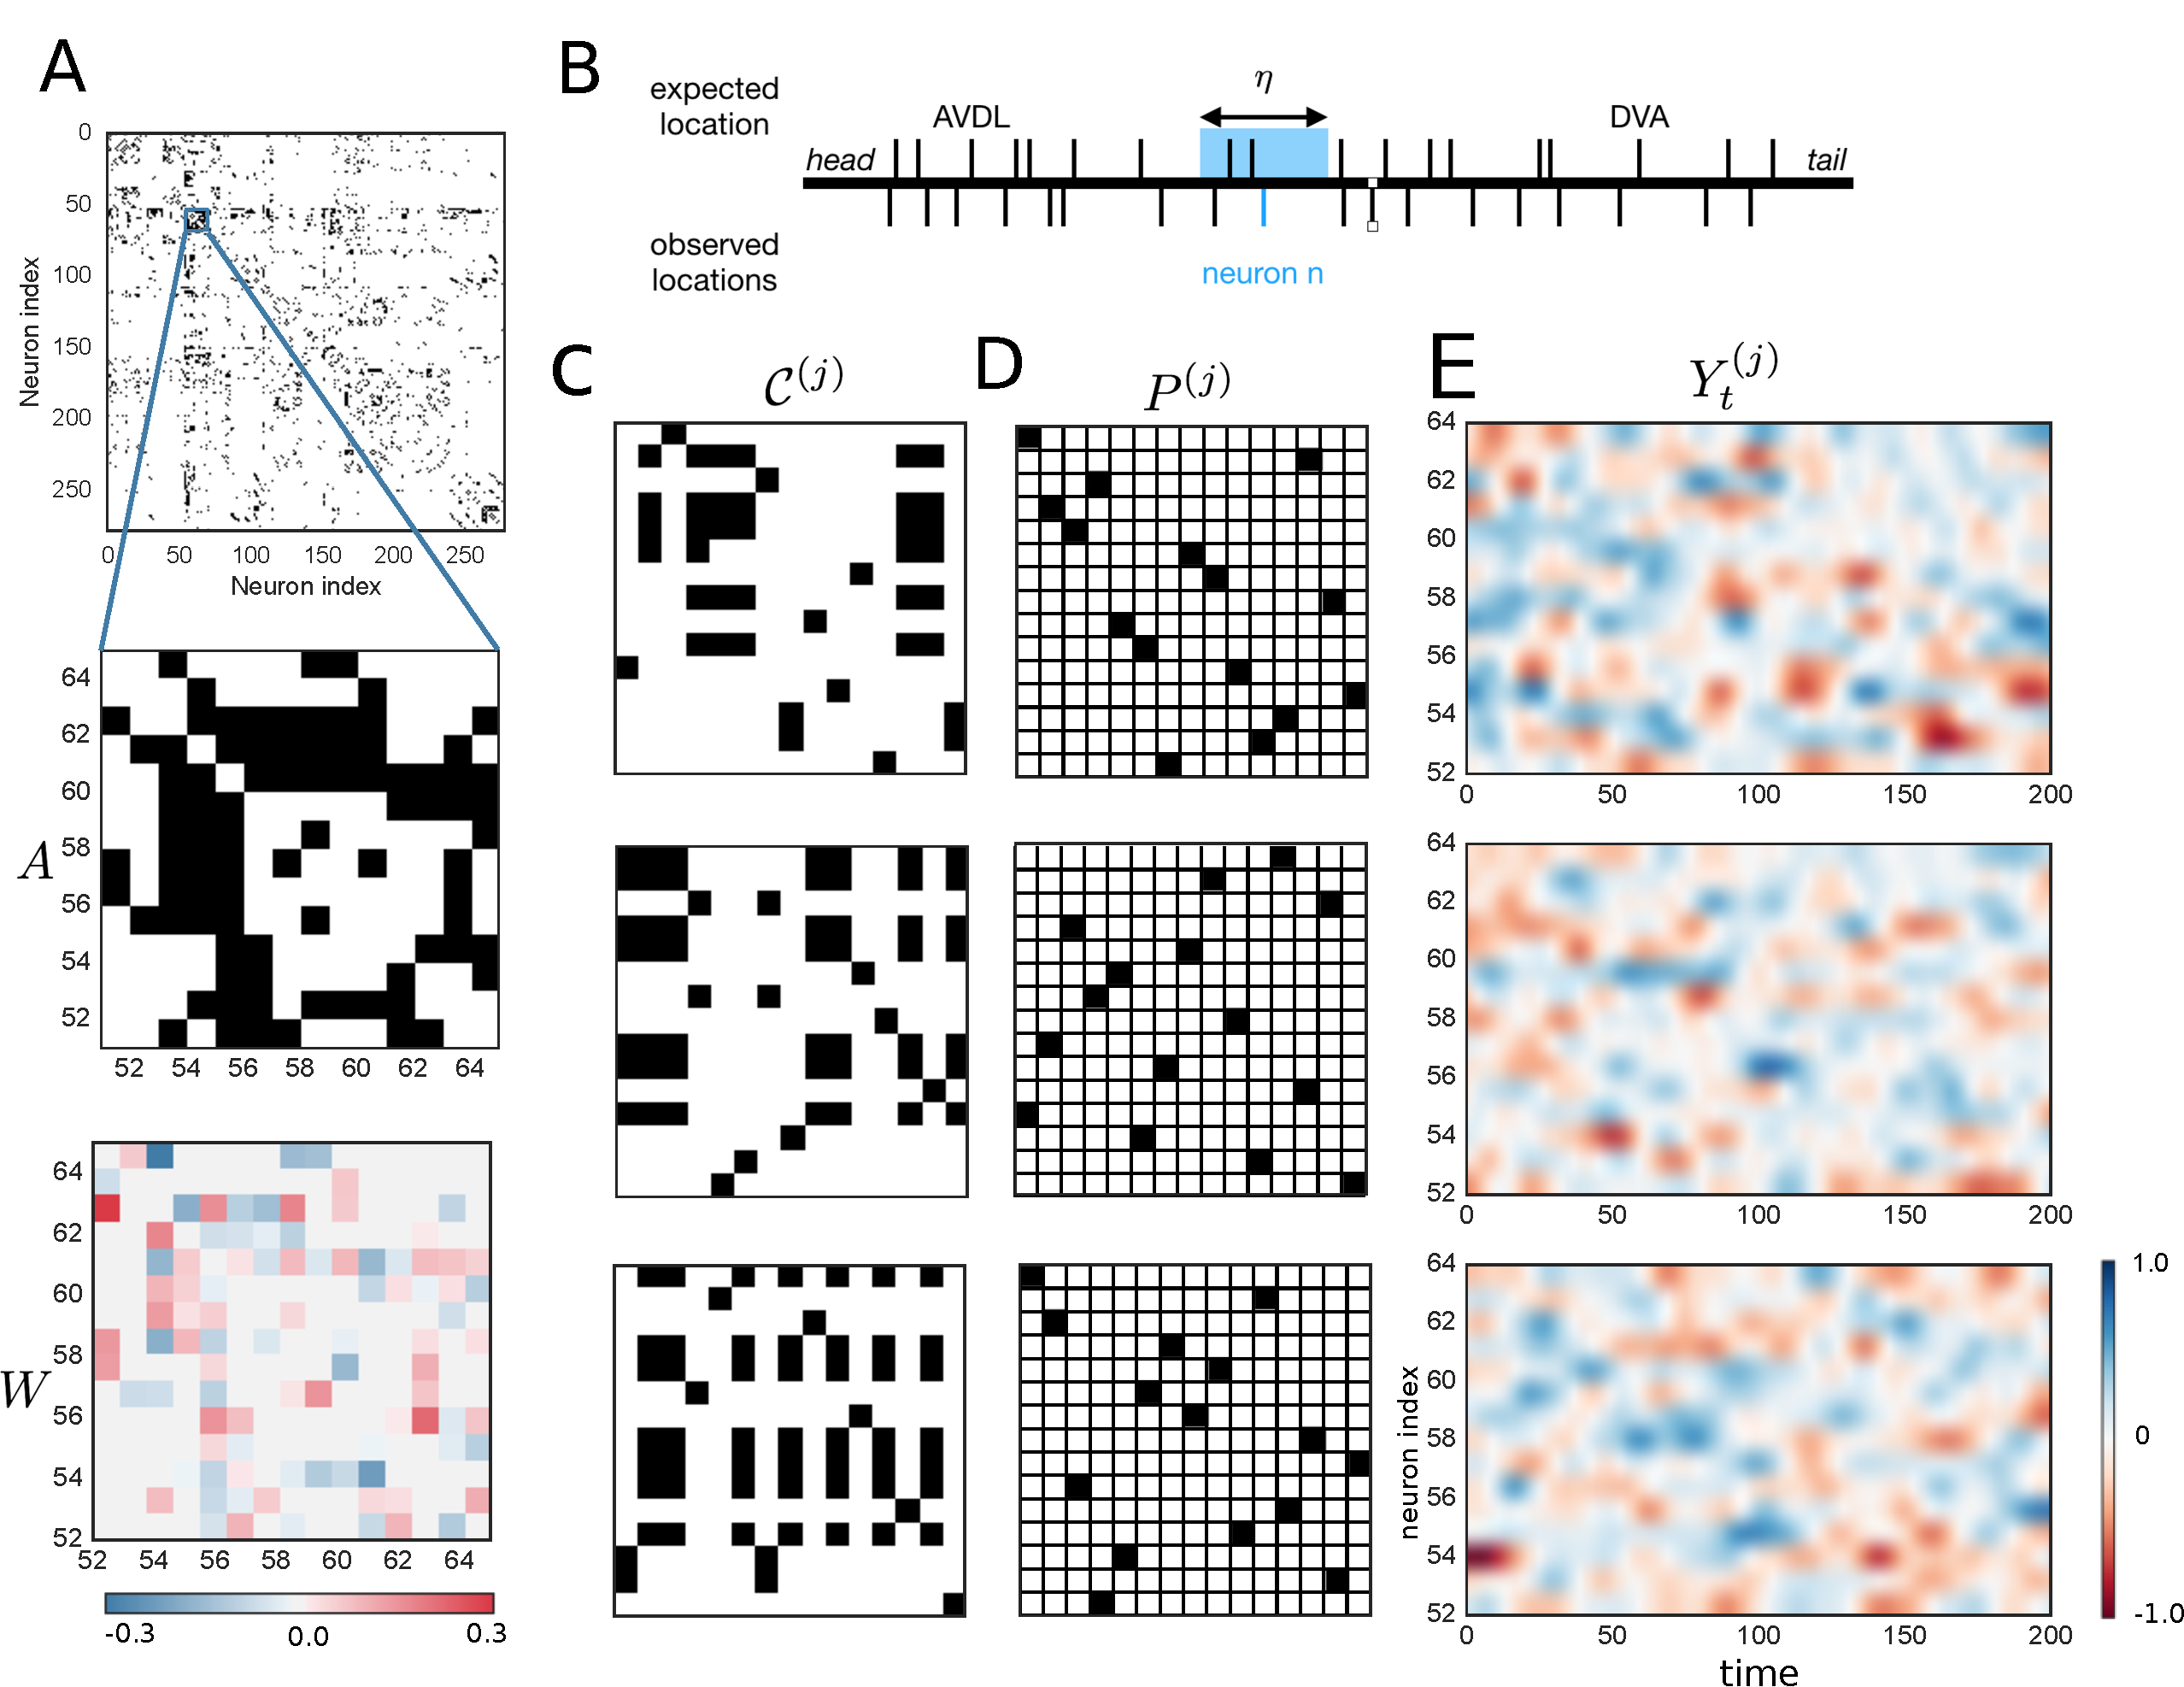
\includegraphics[width=5.0in]{Figure1.pdf} 
  \caption{Hierarchical model outline. \textbf{A} (top) actual connectome $A$, from \citep{varshney2011structural}, (center) zoom-in to 14 neurons, (bottom) sampled matrix $W$ consistent with $A$. \textbf{B} reference linear location information  \citep{white1986structure,wormatlas} can incorporated in our model to constrain posibilities. \textbf{C} in detail, location constrains are represented through a confusion matrix $\mathcal{C}^{(j) }$ that encodes which assignments are possible for each neuron. \textbf{D} permutations $P^{(j)}$ are chosen in consistency with constrains. \textbf{E} dynamical system observations $Y_t^{(j)}$ are sampled from $P^{(j)}$-permuted copies of $W$.}
\label{fig:1}
\end{figure*}


 \section{New methods for variational inference of latent permutations}
  \label{sec:VI}
 Consider a latent variable model  determined by a prior over the latent $z\sim p(z)$ and a likelihood $p(y|z)$ for the observed data $y$. In the VI framework, instead of accessing the perhaps intractable posterior $p(z|y)$ one aims to find the distribution $q(z;\nu)$ among a certain variational family, parameterized by $\nu\in \mathcal{V}$, such that it minimizes its discrepancy with $p(z|y)$. Typically, one considers the KL divergence:
 \begin{equation} \nu^* = \argmin_{\nu\in\mathcal{V}} KL\left(p(z|y)\lVert q(z;\nu)\right).\end{equation}
In turn, one can show that the above problem is equivalent to the maximization of the \emph{evidence lower bound} (ELBO):
 \begin{equation}\label{eq:elbo} \nu^* = \argmax_{\nu\in\mathcal{V}} ELBO(q(z;\nu))\equiv  E_{q(z;\nu)}(\log p(y|z)) - KL(q(z;\nu)\lVert p(z)).\end{equation}
 To maximize equation ~\eqref{eq:elbo} one usually appeals to stochastic optimization methods \citep{Kushner1987}: specifically, all the expectations involved in ~\eqref{eq:elbo} are approximated by Monte Carlo samples, and gradient descent iterations are then performed to this approximation. One critical component is the choice of the Monte Carlo approximation. Perhaps the most common choice is through the so called \emph{score function estimator}, which bases upon the identity $h(\nu) \nabla_\nu \log h(\nu) =\nabla_\nu h(\nu)$. Unfortunately, this estimator, also referred to as REINFORCE \citep{Williams1992}, cannot be applied to permutations, since it involves the evaluation and differentiation of a likelihood which is intractable for any non-trivial distribution over permutations (computing the partition function involves a summation over N! terms).
 
An appealing alternative comes from the re-parameterization trick \cite{Kingma2013}, which leads to a new gradient estimator if one can re-parameterize $z$ as a differentiable function of a noise distribution and the parameters; i.e., if for certain $f$ and $\xi\sim p(\xi)$ one has $z=f(\xi,\nu)$. In the case of discrete random variables a re-parameterization always exists and it is given by the \emph{Gumbel trick} \citep{Papandreou2011,Balog2017}, which states that one can sample from any discrete distribution by perturbing each potential with Gumbel i.i.d noise, and then finding the configuration with the maximum value. Unfortunately, the underlying $f$ to this re-parameterization is the non-differentiable $\argmax$ operator, precluding the use of gradient descent methods.

Recent work by \citep{Jang2016,Maddison2016} proposed a solution to this problem, by replacing the $\argmax$ by a temperature ($\tau$) dependent $\mathrm{softmax}$ approximation, which in the limit  converges to the original $\argmax$. By combining the Gumbel trick with the softmax approximation, they conceived the \emph{Concrete} or \emph{Gumbel-Softmax} distribution, and obtain explicit distribution formulae. Then, they showed one can learn on a discrete latent variable model using the re-parameterization trick and gradient descent, by replacing the original ELBO with the surrogate arising by this continuous relaxation, as long as $\tau$ is chosen in a reasonable range: not too high as it would lead to a degenerate distribution in the simplex; but also not too low, to avoid too high variances of the gradients.

We developed three methods for extending the above to permutations. We name then \emph{stick-breaking}, \emph{rounding} and \emph{Gumbel-Sinkhorn} methods. We refer the reader to sections 3.1 and 3.2 of  \cite{Linderman2017} and section 4 of \cite{Anonymous2018learning} for details, respectively. Here we briefly summarize them: in all of them the primary geometric object is the Birkhoff polytope, the convex hull of permutation matrices, and analog to the probability simplex in this case. For the stick-breaking construction, we generalize to this polytope the one that exists in the simplex \citep{Linderman2015}, surmounting a new complication; of being able to consistently ``break the stick'' while satisfying both the row and column constrains that characterize a doubly stochastic matrix. For the rounding construction, we start by a noise distribution and force it to be close to permutation matrices by pulling them towards the extreme-points of the Birkhoff polytope. Finally, for the Gumbel-Sinkhorn method we notice that the so-called \emph{Sinkhorn operator}, or infinite and successive row and column normalization of a matrix, is a a natural extension of the softmax operator. With this, we are able to conceive the Gumbel-Sinkhorn distribution, which approximates the sampling of a relevant discrete distribution. Importantly, while stick-breaking and rounding yield explicit densities, Gumbel-Sinkhorn does not. However, there are ways to circumvent this difficulty, and overall we observe the latter performs the best.

\section{Results}
\label{sec:results}

We compared against three methods: (i) naive
variational inference, where we do not enforce the constraint that
$X^{(j)}$ be a permutation and instead treat each row of~$X^{(j)}$ as
a Dirichlet distributed vector; (ii) MCMC, where we alternate between
sampling from the conditionals of $W$ (Gaussian) and ${X^{(j)}}$, from
which one can sample by proposing local swaps, as described in
\cite{Diaconis2009}, and (iii) maximum a posteriori estimation (MAP).
Our MAP algorithm alternates between the optimizing estimate of $W$ given~$\{X^{(m)}, Y^{(m)}\}$ using linear regression and finding the optimal ${X^{(j)}}$. The second step requires solving a quadratic assignment
problem (QAP) in ${X^{(j)}}$; that is, it can be expressed as
$\mathrm{Tr}(AXBX^\trans)$ for matrices $A,B$. We used the QAP solver
proposed by~\citet{Vogelstein2015}.


We found that our method outperforms each
baseline, Specifically, we show that our method outperforms alternatives when there are many possible
candidates (Table 1) and when only a small proportion of neurons are known with
certitude (Table 2). 
Altogether, these results indicate our method enables a more efficient
use of information than its alternatives. This is consistent with
other results showing faster convergence of variational inference over
MCMC \citep{Blei2017}, especially with simple Metropolis-Hastings
proposals. We conjecture that MCMC could eventually obtain similar if
not better results, if current local proposals---swapping pairs of
labels--- were replaced by more involved ones.
\begin{table}[h!]
   \centering
  \begin{tabular}{lllllllllll}
    & \multicolumn{2}{c}{10} & \multicolumn{2}{c}{30} &   \multicolumn{2}{c}{45} & \multicolumn{2}{c}{60} \\
    \cmidrule(lr){2-3} \cmidrule(lr){4-5} \cmidrule(lr){6-7} \cmidrule(lr){8-9}
& 1 worm & 4 worms & 1 Worm & 4 worms & 1 worm & 4 worms & 1 worms & 4 worms \\
    \midrule 
    NAIVE VI &.34 & .32 & .16 & .16 & .13 & .12 & .11 & .12 \\
   MAP   & .34 & .32  &.17 &.17& .14 & .13 & .13 & .12 \\
    MCMC   & .34 & .65  &.18 &.28& .14 & .17 & .13 & .15 \\
      %\makecell[l]{Gumbel-Sinkhorn \\ (no regularization)} 
     % &.77 & .92 & \textbf{.4} & .64 &  .25 & .44 & .21 & .39 \\
       %Rounding  (VI) &   .77  & .93 &  .33 &\textbf{.7} &  .18 & .48 & .17 & .37 \\
    VI   & \textbf{.79} & \textbf{.94} & \textbf{.4} & \textbf{.69} & \textbf{.25}&  \textbf{.51} & \textbf{.21} & \textbf{.44}\\
 
    \bottomrule
  \end{tabular}
   \caption{Accuracy in the C.elegans neural identification problem, for varying mean number of candidate neurons (10, 30, 45, 60) and number of worms.}
   \label{table:celeganssup}
\end{table}
\begin{table}[h]
   \centering
  \begin{tabular}{lllllllll}
    & \multicolumn{2}{c}{40.\%} & \multicolumn{2}{c}{30.\%} & \multicolumn{2}{c}{20.\%} & \multicolumn{2}{c}{10.\%}\\
    \cmidrule(lr){2-3} \cmidrule(lr){4-5} \cmidrule(lr){6-7} \cmidrule(lr){8-9}
     & $\eta=0.1$ & $\eta=0.2$ & $\eta=0.1$ & $\eta=0.2$  & $\eta=0.1$ & $\eta=0.2$  & $\eta=0.1$ & $\eta=0.2$ \\
    \midrule 
    Naive VI .43 & .41 & .33 & .31 & .23 & .22 & .12 & .1 \\
    MAP & .42 & .41  &.33 &.32& .23 & .22 & .12 & .11 \\
     MCMC   & .85 & .80  &.52 &.46& .3 & .26 & .15 & .12 \\
   %   \shortstack{Gumbel-Sinkhorn, no regularization (VI)} & .96 & .93 & .88 & .78 &  .69 & .52 & .39 & .21 \\
   %Rounding (VI)& \textbf{.97} & \textbf{.95} & \textbf{.90} & .84 & .75&  .\textbf{58} & \textbf{.37} & \textbf{.17} \\
    VI   & \textbf{.97} & \textbf{.96} & \textbf{.92} & \textbf{.84} & \textbf{.74} & \textbf{.58} & \textbf{.44} & \textbf{.23} \\
              \bottomrule
  \end{tabular}
   \caption{Accuracy in inferring true neural identity for different of proportion of known neurons, and two values of $\eta$. }%\todo[inline]{Gonzalo: Tell the reader what they should take away from these results.  It seems like this significantly outperforms Linderman et al. when there is significantly less data.  Also, with more data the differences don't neccesarily seem that significant.  Why is that the case?  What makes this method better in some circumstances than that one?}}
   \label{table:celegans}
\end{table}
\clearpage

\bibliography{refs}
\bibliographystyle{abbrvnat}

\end{document}
